\subsection{Summary Type Questions}
\label{approach1}
This section describes our efforts to address the ideal answer category on BioASQ along with the description type category of MS MARCO. % where the goal is to produce a query-based, relevant, non redundant and coherent summary answer from multiple snippets and documents. 
We proceeded with this answer type category with the specific hypothesis in mind. They are:
\begin{itemize}
\item Hypothesis 1: A QA system that provides accurate, non-repetitive answers must be supported by a strong Information Retrieval system.
\item Hypothesis 2: Human readability is a harder problem to tackle with. Abstractive methods perform better on this front than the extractive methods	\end{itemize}


 \begin{figure*}
     \centering
     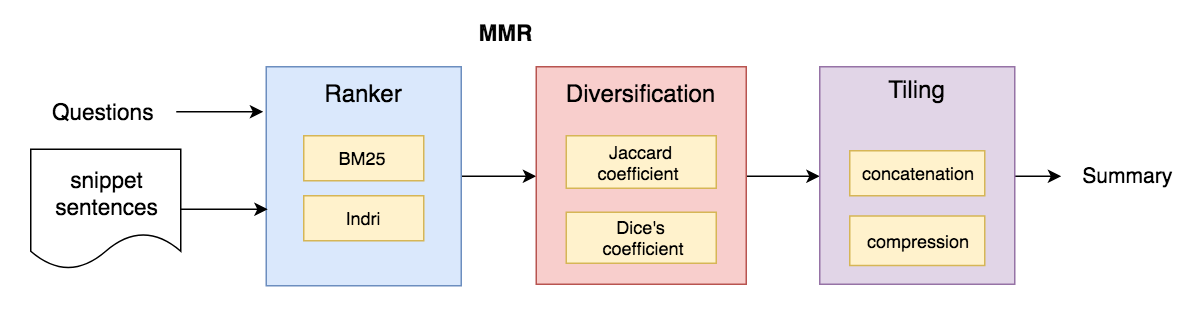
\includegraphics[scale=0.3]{images/pipeline_summary.png}
     \caption{Pipeline for ideal answer generation}
     \label{fig:ideal_answers_pipeline}
 \end{figure*}
\subsubsection{Extractive summarization}
Our pipeline for ideal answers has three stages. The first stage involves pre-processing of answer snippets and ranking of answer sentences by various retrieval models described in the following sections. The retrieval model scores form the soft positional component introduced in the MMR algorithm. We perform sentence selection next, where we select the top 10 best sentences for generating an ideal answer. The third and final stage involves tiling together the selected sentences to generate a coherent, non redundant, ideal answer for the given question. 
 %We describe our improvements to the pipeline that can be applied to all the above categories with primary focus being summary type questions as described in Section \ref{Dataset}.
The subsequent subsections explain the full pipeline for ideal answer type questions in detail (see Figure \ref{fig:ideal_answers_pipeline}).

\subsubsection{Question-Sentence Retrieval}
In this section we describe various approaches which were adapted to improve the initial retrieval of candidate sentences. We used the standard BM25 algorithm with custom pre-processing to exclude medical entities from stop word removal.  

\subsubsection*{BM25}
BM25 \cite{BM25} is a standard tf-idf based retrieval algorithm relying on bag of words approach for document retrieval. We considered every question to be independent and built an inverted index over the relevant snippets following the standard methods. Since the snippets are short paragraphs and the question is of moderate length, we tuned BM25 parameters accordingly. We customized the pre-processing by creating our own set of stop words that excluded certain bio-medical entities which might have been considered an English stop-word.

\[Score(D, Q) = \sum_1^n IDF(q_i) \frac{f(q_i, D) (k_1 + 1)}{f(q_i, D) + k_1 (1- b + b . \frac{|D|}{avgdl})} \]



\subsubsection*{Indri}

Indri \cite{Indri} is more modern retrieval model based on the use of statistical language models and query likelihood. We assumed a uniform prior over the sentences and ranked the candidate sentences based on the probability of the question given the sentence. 
We employed a two-stage smoothing that considers characteristics of both the query (the question in this context) and answer sentences. 

The Indri score for a candidate sentence is estimated in a collection (C) of snippets as follows:
\begin{align}
    & p(q_i|d) = (1-\lambda) p_{mle} (q_i|d) + \lambda p_{mle} (q_i|C) \label{eq1} \\ 
    & p_{mle}(q_i|d) = 
    \frac{tf + \mu  p_{mle}(q_i|C)}{length(d) + C} \label{eq2} \\ 
    & p_{mle}(q_i | C) = \frac{ctf}{length(C)}
\end{align}

where, $\lambda$ is the coefficient for linear interpolation based smoothing that accounts for question length smoothing. Since the questions are of moderate length, after tuning, the best value of $\lambda$ is attained at 0.75

In equation \ref{eq2}, $\mu$ is parameter for Bayesian smoothing using Dirichlet priors used for sentence length normalization. Since sentences of snippets can be of varying lengths, after tuning, the best value of $\mu$ is attained at 5000.

Both of the above smoothing techniques do two different things, the mixture model (interpolation) compensates for differences in the word importance (gives idf-effects) and the Dirichlet prior improves the estimates of the sentence sample which supports our decision to use two stage smoothing. 

% \subsubsection{LeToR}

% Learning to Rank \cite{Letor} is widely used, supervised learning approach for ranking the candidate sentences. We propose a new technique to create gold data for training the LeToR model. For every training data sample, we created a golden ranking of the sentences by ranking the candidate sentences from all the given snippets using golden ideal answer as the question following BM25 algorithm. For feature engineering part of LeToR, we considered different semantic, statistical and language model based features.
% \begin{itemize}
%     \item \textbf{Tf-Idf based}: BM25 score of the sentence
%     \item \textbf{Language model based}: Indri score of the sentence
%     \item \textbf{Semantic}: Count of the Named Entities in each sentence.
%     \item \textbf{Biomedical entities}: We obtained the biomedical entities from biomedical entity extraction tools like PubTator \cite{pubtator}, Lingpipe \cite{lingpipe} and GramCNN \cite{gramcnn}.
% \end{itemize}
% BM25, Indri algorithms were adapted as features for LeToR which was our final model for ranking candidate sentences


\subsection{Sentence Selection}
Once the top most relevant snippets have been chosen, we want to choose sentences from these snippets which are most relevant to a specific question. In this section we demonstrate how this selection is done.

\subsubsection{MMR}

We use the Maximum Marginal Relevance (MMR) algorithm \cite{MMR} as the baseline for sentence selection. In contrast to the basic Jaccard similarity metric used in previous work \cite{khyati-paper}, we experimented with other similarity measures which consistently perform better than the Jaccard baseline. MMR ensures the selected set contains non-redundant yet complete information. The sentences are selected based on two aspects, the sentence's relevance to the question and how different it is to the already selected sentences. At each step we select a document to append to the ranking based on the equation below.
\vspace{-0.3cm}
\begin{equation}
     d_i = \argmax_{d_j\in R \setminus S} (\lambda \cdot sim(q, d_i)  - (1 - \lambda) \cdot max\limits_{d \in \mathcal{S}}(sim_{sent}(d_i, d_j) ) ) \label{eq4}
\end{equation}
   

 We define a custom similarity metric between documents which uses positional values of sentences from the initial ranking as follows:
 \vspace{-0.3cm}
\begin{equation}
  sim_{sent}(di, dj) = ( 1 - \beta) \cdot (1 - \frac{rank(s_i)}{n}) + \beta \cdot sim(d_i, d_j) 
\end{equation}
Here, $sim_{sent}(di, dj)$ is the sentence to sentence similarity, $sim(q, di)$  is the question - sentence similarity, $rank(s_i)$ is the rank of the snippet which contains the sentence $d_i$, $S$ are Sentences already selected for summary i.e. which are ranked above this position. In the above equation, we tried various metrics to account for the sentence to sentence similarity. In cases where $\beta$ is non-zero, equation \ref{eq4} is identified as our SoftMMR which includes soft scoring based on sentence position.

\subsubsection{Dice's similarity Coefficient (DSC)}

Dice's similarity Coefficient (DSC) \cite{dice} is a quotient of similarity between two samples and ranges between 0 and 1 calculated as
It is used to compare similarity of two strings using bigrams. It is different from the Jaccard coefficient which counts intersecting words only once in both the numerator and denominator. 

\begin{equation*}
    dsc = \frac{(2 * n_t)}{ (n_x + n_y)}
\end{equation*}
where $n_t$ is the number of character bigrams found in both strings, $n_x$ is number of bigrams in string $x$ and $n_y$ is the number of bigrams in string $y$.
\subsection{\textbf{Evaluation}}
\subsubsection{BioASQ} 
The pipeline described above is primarily designed to improve the ROUGE evaluation metric \cite{Rougue}. Although a higher ROUGE score does not necessarily reflect improved human readability, MMR can improve readability by reducing redundancy in generated answers.
Results for ideal answers for Task 5 phase b for BioASQ dataset are shown in Table \ref{tab:rouge_extractive_summarization}. We also compare our results with other state of the art approaches in Table. Based on the results we accept our hypotheses 1 that a QA system needs to have strong IR  \ref{tab:comparison_results}.
\subsubsection{MS MARCO}
Now coming to the MS MARCO description dataset, the same pipeline couldn't be applied as is. Summary of BioASQ and Description of MS Marco are not exactly the same. Summary of BioASQ can be seen a subset of Description. The main difference being the average length of the description type answers. As mentioned in the dataset statistics, considering the number of sentences and average sentence length, we changed the number of words in summary from 200 to 20-25. That significantly improved our BLEU. Also, please note that we have performed the experiments on a smaller sample of the data. The results for description type questions are seen in the table \ref{tab:ms_marco_ext_res}.

\begin{table}[t!]
    \centering
    \begin{tabular}{|l|c|c|c|}
         \hline
            $\beta$& Configuration & Rouge-2 & Rouge-SU4 \\
        \hline
        \hline
        - & baseline & 0.7064 & 0.6962 \\
        \hline
        0.5 & BM25, Jaccard  & 0.7175 & 0.7110  \\ 
        \hline
        0.5 & BM25, Dice & 0.7193 & 0.7106  \\ 
        \hline
        0.6 & BM25, Dice & 0.7133 & 0.7053  \\ 
        \hline
        0.6 & BM25, Jaccard & 0.7133 & 0.7053  \\
        \hline
        \textbf{0.5} & \textbf{ Indri, Jaccard} & \textbf{0.7206} & \textbf{0.7135}  \\ 
        \hline
         0.5 & Indri, Dice & 0.7113 & 0.7052  \\ 
        \hline
    \end{tabular}
    \caption{ROUGE scores for different experiments on similarity metrics for extractive summarization}
    \label{tab:rouge_extractive_summarization}
\end{table}

\begin{table}[t]
    \centering
    \begin{tabular}{|c|c|c|c|c|} \hline
    \textbf{Configuration} & \textbf{Bleu 1} & \textbf{Bleu 2} & \textbf{Bleu 3} & \textbf{Rouge-L} \\
    \hline
      Wordlimit = 25, BM25, DuoSimilarity & 0.215 & 0.139 & 0.109 & 0.175\\
     \hline
     Wordlimit = 50, BM25, DuoSimilarity &  0.206 & 0.108 & 0.093 & 0.162\\
    \hline
    \end{tabular}
    \caption{Results on the MS Marco dataset}
    \label{tab:ms_marco_ext_res}
\end{table}

\subsubsection{Abstractive Summarization}
Neural sequence-to-sequence models have provided a viable new approach for abstractive text summarization insteas of simply selecting and rearranging passages/sentences from the original text. However, these models have a problem where the summary generated looks like sentences stitched together and not readable as if generated by a human.To address this, we tried Pointer Generator Networks as mentioned in \cite{PGC}

However, we couldn't get the expected results due to multiple reasons. We used a pretrained model which was trained on CNN daily mail data which lead to many UNKs (Unknown words) due to difference in the Vocabulary. Also we didn't add the coverage mechanism for penalizing repetitive sentences. This is a direction for our future work.

\subsubsection{Error Analysis}
\begin{itemize}
    \item Case 1: When the question asks to describe a very specific aspect/ affect. \\
    E.g.: \textit{What causes genetic alterations in normal cells ?}
    Here the question asks to narrow a specific reason that explains a scenario. The answer generated by the system spoke about genetic alterations in normal cells and its characteristics but not causes.
    \item Case 2: When the answer is beyond the understanding of the question and content at a surface level. \\
    E.g.: \textit{Why is albumin normally absent in urine?} Here, the system can't understand that it has to understand the word 'absent' and not match the sentences which has either only albumin or urine in it in a different context.  
    \item Case 3: Inference type of questions. \\
    E.g.: \textit{A went to New York and bought a house. Where is the house?}
    System couldn't infer that the house is in NY.
\end{itemize}